\section{RNA-Seq: QC/QA post alignment}
Although we have ensured the base quality of our reads is high, there may be many other factors we did not look into because they can only be deduced from the alignments.
There are several tools available to check for certain biases within alignments.

\subsection{CollectRnaSeqMetrics}
For this module, load the Shared Data (\textit{\datalibrarydirrnaseqadvanced}) files:\\
``paired-end-rna-seqmetrics.bam'' and ``ucsc\_refseq.gtf'' and proceed with the tool \textit{CollectRnaSeqMetrics} as follows:\\
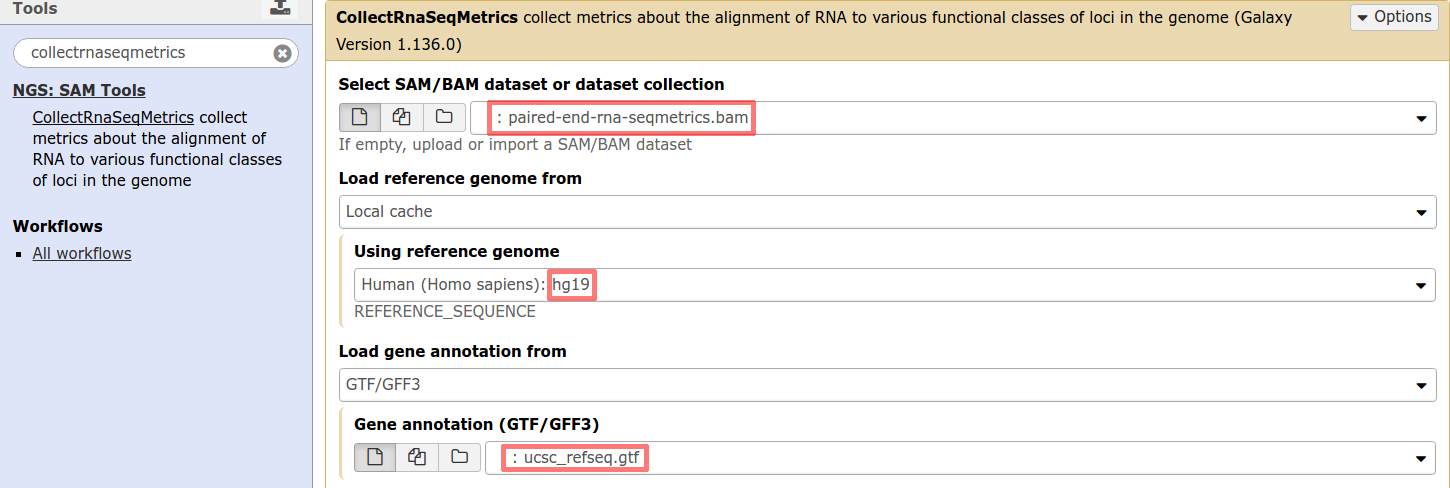
\includegraphics[width=\textwidth]{figures/qc2_01.png}\\
This analysis will take a while (2 minutes) and will return two files, a summary file and a PDF file.
Take a look at the PDF.
This pictures shows the average coverage per relative position within all genes.
As you can see there is a bias towards the 5' end.
This means that overall more reads are aligned to the 5' end of the genes, due to library preparation.
For certain types of analysis (e.g. differential isoform expression analysis) it might be important to keep this information in mind.

\subsection{Inner Distance}
% The one of RSeqC gives a clearer report than the one of Picard
For this module, add the Shared Data (\textit{\datalibrarydirrnaseqadvanced}) file:\\
``refseq-genes.bed'' and proceed with the tool \textit{Inner Distance} as follows:\\
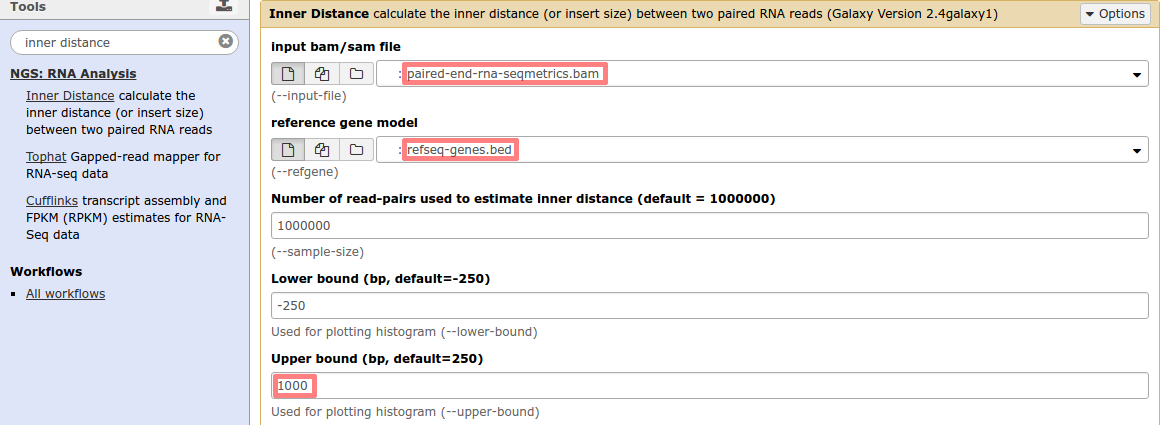
\includegraphics[width=\textwidth]{figures/qc2_02.png}\\
The insert size is the size of the original cDNA fragment (minus the length of the mate pairs).
Because RNA-seq fragments are size selected, the fragments should be within a certain range, usually provided by the manufacturer.
An easy way to estimate this is by calculating the insert size, the distance in between the mates.
However, due to the gaps introduced by introns in RNA-Seq, the insert size may be much larger than the actual fragment size.
The tool \textit{Inner Distance} corrects for splice junctions in the alignments and makes a plot of the distribution of the insert sizes.
When you take a look at the result, you will first need to understand the $x$-axis.
If the length of the both mates of a read is 100bp, and the insert size in the figure is 0, the length of the RNA fragment was $100+0+100=200$nt.
If the insert size in the figure is 25 (mean) and both mates are 100bp in length, the RNA fragment was $100+25+100=225$nt.
Given that the mean of the insert size is $\sim25$bp, the most abundant fragment size is $225$nt.

Let's assume the manufacturer said that the fragments are size selected between 200 and 500bp.
You should be able to understand why there are insert sizes smaller than 0 (insert size smaller than 200) but also why they can be larger (technical and biological).
% Biological: indels
% Technical:
% - Quality trimming of reads
% - Mistakes in protocol - size selection and fragmentation
There is also a small bulb of reads with an insert size even smaller than the fragment (200bp), meaning a negative fragment size.
Of course, this is not possible.
These are reads of which the forward mate is aligned after the reverse.

%\subsection{Clipping Profile}
